
\begin{IEEEbiography}[{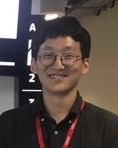
\includegraphics[width=1in,height=1.25in,clip,keepaspectratio]{figures/author_krk}}]{Kyurae~Kim} (Student Member, IEEE) received the B.S. degree in electronics engineering from Sogang University, Seoul, South Korea, in 2021.

  He worked as an undergraduate researcher at Samsung Seoul Hospital, Seoul, South Korea from 2017 to 2020.
  He currently works as a Research Associate at the Department of Electrical Engineering and Electronics, University of Liverpool, Liverpool, United Kingdom.
  His research interests include Bayesian inference methods, probabilistic machine learning, parallel computing, and image processing.
\end{IEEEbiography}

\begin{IEEEbiography}[{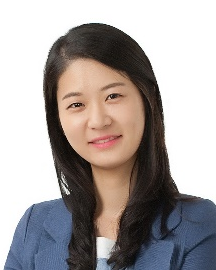
\includegraphics[width=1in,height=1.25in,clip,keepaspectratio]{figures/author_mrl}}]{Miran Lee} received the B.S. degree in Health Science from Korea University, Seoul, South Korea, in 2008, and the M.S. degree from the Department of Biomedical Sciences, Korea University, Seoul, South Korea, in 2014.

  She has been working as a Cardiac Sonographer at the Department of Total Healthcare Center, Kangbuk Samsung Hospital, Sungkyunkwan University School of Medicine, since 2013.
  She is currently a Ph.D. student in Electronics Engineering at Sogang University. 
  Her main research interests are in developing efficient artificial intelligence architectures for ultrasound systems and deep learning in medical images.
\end{IEEEbiography}

\begin{IEEEbiography}[{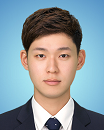
\includegraphics[width=1in,height=1.25in,clip,keepaspectratio]{figures/author_kkl}}]{Kunkyu Lee}
received the B.S. and M.S degrees from the Department of Electronic Engineering, Sogang University, Seoul, South Korea, in 2016 and 2018, respectively.

He is currently a Ph.D. student in Electronics Engineering at Sogang University.
His main research interests are the development of efficient portable ultrasound imaging system, the efficient architecture of artificial intelligence with ultrasound system and Deep learning image processing in medical images.
\end{IEEEbiography}

\begin{IEEEbiography}[{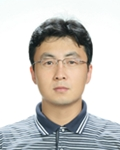
\includegraphics[width=1in,height=1.25in,clip,keepaspectratio]{figures/author_mk}}]{Min Kim} received the Ph.D. degree in the Department of Electronic Engineering, the Sogang University, Seoul, South Korea. 

From 2017 to 2019, he worked as a research professor of the Department of Electronic Engineering, Sogang University. 
He is currently the Director of the Research Institute of Hansono, Seoul, South Korea. 
His research interests include ultrasound image processing and hand-held ultrasound systems for point-of-care ultrasound.
\end{IEEEbiography}

\begin{IEEEbiography}[{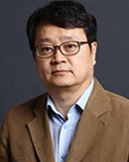
\includegraphics[width=1in,height=1.25in,clip,keepaspectratio]{figures/author_tks}}]{Tai-kyong Song} (Member, IEEE) received the B.S. degree in electronic engineering from Sogang University, Seoul, South Korea, in 1984, and the M.S. and Ph.D. degrees from the Department of Electrical and Electronic Engineering, Korea Advanced Institute of Science and Technology (KAIST), Seoul, in 1985 and 1990, respectively. 

  He worked as a Research Fellow at the Department of Physiology and Biophysics, Mayo Clinic, Rochester, MN, USA, for two years before appointed as an Adjunct Professor with the Department of Information and Communication Engineering, KAIST, from 1993 to 1995.
  He worked as a Staff Scientist at Siemens Healthcare, Medical-System Inc., Issaquah, WA, USA, from 1995 to 1997.
  He joined the Department of Electronic Engineering, Sogang University as an Assistant Professor, in 1997.
  He was promoted to a professor, in 2006. He has been the Director of the Medical Solution Institute, Sogang University, since 2000.
  His research interests include medical ultrasound imaging and therapy, portable ultrasound imaging systems, ultrafast 3-D scanning algorithms, photoacoustic imaging and its translational research, digital signal and image processing, and multimodal imaging system for preventive and surgical applications.
  He is currently the President of the Korean Medical Ultrasound Link, South Korea.
  He has served as an Associate Editor for the \textsc{IEEE Transactions on Ultrasonics, Ferroelectrics, and Frequency Control}, from 2002 to 2007.

  Prof. Song is a member of the National Academy of Engineering of Korea (NAEK), South Korea. 
\end{IEEEbiography}

%%% Local Variables:
%%% TeX-master: "master"
%%% End:
